\documentclass[12pt, twosided]{article}

\usepackage[letterpaper,bindingoffset=0in,%
            left=1in,right=1in,top=1in,bottom=1in,%
            footskip=.25in]{geometry}

\usepackage{mathtools}
\usepackage{graphicx}

\usepackage{setspace}
\setstretch{1.1}

\usepackage{amsmath}
\usepackage{amsfonts}
\usepackage{amsthm}
\usepackage{amssymb}
\usepackage{csquotes}
\usepackage{relsize}

\usepackage{tikz}
\usetikzlibrary{cd}
\usetikzlibrary{fit,shapes.geometric}
\tikzset{%  
    mdot/.style={draw, circle, fill=black},
    mset/.style={draw, ellipse, very thick},
}

\usepackage{hhline}
\usepackage{systeme}
\usepackage{mathrsfs}
\usepackage{hyperref}
\usepackage{mathtools}  
\usepackage{silence}
\usepackage{blkarray}
\usepackage{float}
\usepackage{framed}
\usepackage{array}
\usepackage{stmaryrd}
\usepackage{extarrows}
\usepackage{caption}
\captionsetup[figure]{labelfont={bf},name={Fig.},labelsep=period}

\theoremstyle{definition}
\newtheorem{df}{Definition}
\newtheorem{exa}{Example}
\newtheorem{ques}{Question}
\newtheorem{exr}{Exercise}
\newtheorem*{note}{Note}
\theoremstyle{plain}
\newtheorem{thm}{Theorem}
\newtheorem{prop}{Proposition}
\newtheorem{conj}{Conjecture}
\newtheorem{cor}{Corollary}
\newtheorem{lm}{Lemma}
\newtheorem*{fact}{Fact}
\newtheorem*{idea}{Idea}
\newtheorem*{clm}{Claim}
\newtheorem*{rmk}{Remark}
\usepackage[ruled]{algorithm2e}

\usepackage{ulem}
\makeatletter

\def\lf{\left\lfloor}   
\def\rf{\right\rfloor}
\def\lc{\left\lceil}   
\def\rc{\right\rceil}
\def\st{\text{ s.t. }}
\def\1{^{-1}}
\def\ind{\mathbf{1}}
\def\R{\mathbb{R}}
\def\Q{\mathbb{Q}}
\def\Z{\mathbb{Z}}
\def\C{\mathbb{C}}
\def\I{\mathbb{I}}
\def\N{\mathbb{N}}
\def\F{\mathbb{F}}
\def\A{\mathbb{A}}
\def\Li{\text{Li}}
\def\th{^\text{th}}
\def\sp{\text{Sp}}
\def\opn{\left\{}
\def\cls{\right\}}
\def\Aut{\text{Aut}}
\def\PG{\text{PG}}
\def\GL{\text{GL}}
\def\PGL{\text{PGL}}
\def\Cov{\text{Cov}}
\def\Pack{\text{Pack}}
\def\PgamL{\text{P}\Gamma\text{L}}
\def\gamL{\Gamma\text{L}}
\def\cl{\text{cl}}
\def\stbar{\ \middle\vert\ }
\def\partdone{\hphantom{1} \hfill \(\triangle\)}
\def\s0{_0}
\def\s1{_1}
\def\s2{_2}
\def\id{\mathrm{id}}
\def\topn{\text{ open}}
\def\Bd{\text{Bd }}
\renewcommand{\P}{\mathbb{P}}
\newcommand{\leg}[2]{\left( \frac{#1}{#2} \right)}
\renewcommand*\env@matrix[1][*\c@MaxMatrixCols c]{%
   \hskip -\arraycolsep
   \let\@ifnextchar\new@ifnextchar
   \array{#1}}
\makeatother

% These two lines suppress the warning generated 
% by amsmath for overwriting the choose command  
% because it's annoying. This probably has unint-
% ended ramifications somewhere else, but I'm too
% lazy to actually figure that out, so we'll cro-
% ss that bridge when we come to it lol.
\renewcommand{\choose}[2]{\left( {#1 \atop #2} \right)}
\WarningFilter{amsmath}{Foreign command} 

\renewcommand{\mod}[1]{\ (\mathrm{mod}\ #1)}
\renewcommand{\vec}[1]{\mathbf{#1}}

\let\oldprime\prime
\def\prime{^\oldprime}

\usepackage{float}
\restylefloat{figure}

\usepackage{cleveref}
\Crefname{thm}{Theorem}{Theorems}

% Comment commands for co-authors
\newcommand{\kmd}[1]{{\color{purple} #1}}

\newcolumntype{L}{>{$}l<{$}}
% Bib matter
\let\oldepsilon\epsilon
\def\epsilon{\varepsilon}

\let\oldphi\phi
\def\phi{\varphi}

%%% Local Variables:
%%% mode: plain-tex
%%% TeX-master: t
%%% End:

\graphicspath{{./img/}}

\begin{document}
\noindent \textbf{Math 171} \hfill \textbf{Professor Sebastian Bozlee} \\
\textbf{Scribed by: Kyle Dituro} \hfill \textbf{March 10, 2023}\hrule
\vspace{.2in}

Let's go over part (b) of the early problem...

\begin{prop}
  Let \(X, Y\) be topological spaces, and let \(\mathcal{B}_X, \mathcal{B}_Y\) be bases for the resp. topologies of \(X, Y\), then:

  \begin{enumerate}
  \item \(f: X \to Y\) is continuous iff for each \(B \in \mathcal{B}_Y\), \(f\1(B)\) is open.
  \item \(f: X \to Y\) is continuous iff for all \(x \in X\) and basic open neighborhoods \(B_{f(x)}\) of \(f(x)\), there exists \(B_x \in \mathcal{B}_x\) such that \(x \in B_x\) and \(f(B_x) \subseteq B_{f(x)}\).
  \end{enumerate}
\end{prop}
The proof of (a) is left to the early problem
\begin{proof}[Proof of part b]
  \begin{enumerate}
  \item [(\(\Rightarrow\))] Let \(f: X \to Y\) be continuous. Let \(x \in X\), and \(B_{f(x)}\) be a basic open neighborhood of \(f(x)\). Then, since \(f(x) \in B_{f(x)}\), \(x \in f\1(B_{f(x)})\). Since \(f\) is continuous, \(f\1(B_{f(x)})\) is open. By the definition of open in a generated topology, \(\exists B_X \in \mathcal{B}_X\) such that \(x \in B_X\) and \(B_x \subseteq f\1(B_{f(x)})\). Then, using the Galois connection, we get that \(f(B_X) \subseteq B_{f(x)}\).
  \item [(\(\Leftarrow\))] Assume that we have the property, now we want to show that \(f: X \to Y\) is continuous. So let \(U \subseteq Y\) be an open set. Now let \(x \in f\1(U)\) Then \(f(x) \in U\). Since \(U\) is open, there is a basic open neighborhood \(B_{f(x)}\) such that \(f(x) \in B_{f(x)}\) and \(B_{f(x)} \subseteq U\). By assumption, there is a basic open neighborhood \(B_x\) of \(x\) such that \(f(B_x) \subseteq B_{f(x)} \subseteq U\). Then again by the Galois connection, \(B_x \subseteq f\1(U)\).
  \end{enumerate}
\end{proof}

  Now on to more stuff.

  \begin{df}
    A set \(S\) of subsets of a set \(X\) whose union is all of \(X\) is a \textbf{subbasis for a topology on \(X\)}. The \textbf{topology generated by \(S\)} is the set of unions of finite intersections of elements of \(S\).
  \end{df}

  We claim that in order to show that this is a topology, it is enough to show that the set \(\mathcal{B}\) of finite intersections of elements of \(S\) is a basis. Now let's actually do the check:

  \begin{proof}
    \begin{enumerate}
    \item Let \(x \in X\). Then since \(\bigcup_{T \in S} T = X\), there is an element \(T \in S\) such that \(x \in T\), and thus \(T \in \mathcal{B}\).
    \item Let \(B_1 = T_1 \cap \ldots \cap T_n\), where \(T_i \in S\), and \(B_2 = T\prime_1 \cap \ldots \cap T\prime_m\), where \(T_i\prime \in S\). Now let \(x \in B_1 \cap B_2\). Since \(B_1 \cap B_2\) is a finite intersection of elements of \(S\), it is a basis element, and so we can take \(B_3 = B_1 \cap B_2\).
    \end{enumerate}
  \end{proof}

  So where is this useful? We will now move into a discussion of product spaces. This is where all of the universal property juggling should pay off.

  \begin{ques}
    Given two topological spaces \(X, Y\), what topology ``should'' we put on \(X \times Y\)?

    More generally, given topological spaces \(X_i\) for \(i \in I\), what topology should \(\prod_{i \in I} X_i\) have?
  \end{ques}

  Let's recall the universal property of the product for sets, and amend it for topological spaces.
  \begin{thm}
    Given \sout{sets} {\color{red} topological spaces} \(X, Y\), a \sout{set} {\color{red} topological spaces} \(P\) together with \sout{functions} {\color{red} continuous functions} \(\pi_1: P \to X\) and \(\pi_2: P \to Y\) is said to have the universal property if, for any \sout{set} {\color{red} topological spaces} \(Z\) and \sout{functions} {\color{red} continuous functions} \(f_1: Z \to X\) and \(f_2: Z \to Y\) there exists a unique \sout{function} {\color{red} continuous function} \(f: Z \to P\) such that.

    \begin{center}
      \begin{tikzcd}
        & Z \arrow[dl, "f_1"] \arrow[dr, "f_2"] \arrow[dotted, d, "\exists! f"] & \\
        X & P \arrow[l, "\pi_1"] \arrow[r, "\pi_2"]& Y
      \end{tikzcd}
    \end{center}
  \end{thm}
  \begin{prop}
    ``Products are unique up to unique homeomorphism.''
    i.e. Given \((P, \pi_1, \pi_2)\) and \((P\prime, \pi_1\prime, \pi_2\prime)\) with the universal property, there exists a unique homeomorphism \(\phi: P \to P\prime\) such that \(\pi_1 = \pi_1\prime \circ \phi\) and \(\pi_2 = \pi_2\prime \circ \phi\). 
  \end{prop}
  \begin{proof} Let's do some good old-fashioned diagram chasing.
    \begin{center}
      \begin{tikzcd}
        & Z \arrow[dl, "\pi_1"] \arrow[dr, "\pi_2"] \arrow[dotted, d, "\exists! \phi"] & \\
        X & P\prime \arrow[l, "\pi_1\prime"] \arrow[r, "\pi_2\prime"]& Y
      \end{tikzcd}
      \begin{tikzcd}
        & Z \arrow[dl] \arrow[dr] \arrow[dotted, d, "\psi"] & \\
        X & P \arrow[l] \arrow[r]& Y
      \end{tikzcd}
    \end{center}
    Combining these two diagrams, we get:
    \begin{center}
      \begin{tikzcd}
        & Z \arrow[dl, "\pi_1"] \arrow[dr, "\pi_2"] \arrow[d, "\psi \circ \phi"] & \\
        X & P \arrow[l, "\pi_1"] \arrow[r, "\pi_2"]& Y
      \end{tikzcd}
    \end{center}
    So then \(\psi \circ \phi\) is the identity map, and we have what we need.
  \end{proof}
    So we can revise our goal: We now want to find a topology on \(X \times Y\) so that \((X \times Y, \pi_1, \pi_2)\) has the universal property.

    In other words, we want to find a topology on \(X \times Y\) such that \(
    \begin{matrix}
      \pi_1: X \times Y \to X \\ (x, y) \mapsto x
    \end{matrix}
    \) and \(
    \begin{matrix}
      \pi_2: X \times Y \to Y \\ (x, y) \mapsto y
    \end{matrix}
    \) are continuous.

    So we need
    \begin{enumerate}
    \item For each \(U \subseteq X\) open, \(\pi_1\1(U) = U \times Y\) is open
    \item For each \(V \subseteq Y\) open, \(\pi_2\1(V) = X \times Y\) is open.
    \end{enumerate}

    \begin{figure}[h]
      \centering
      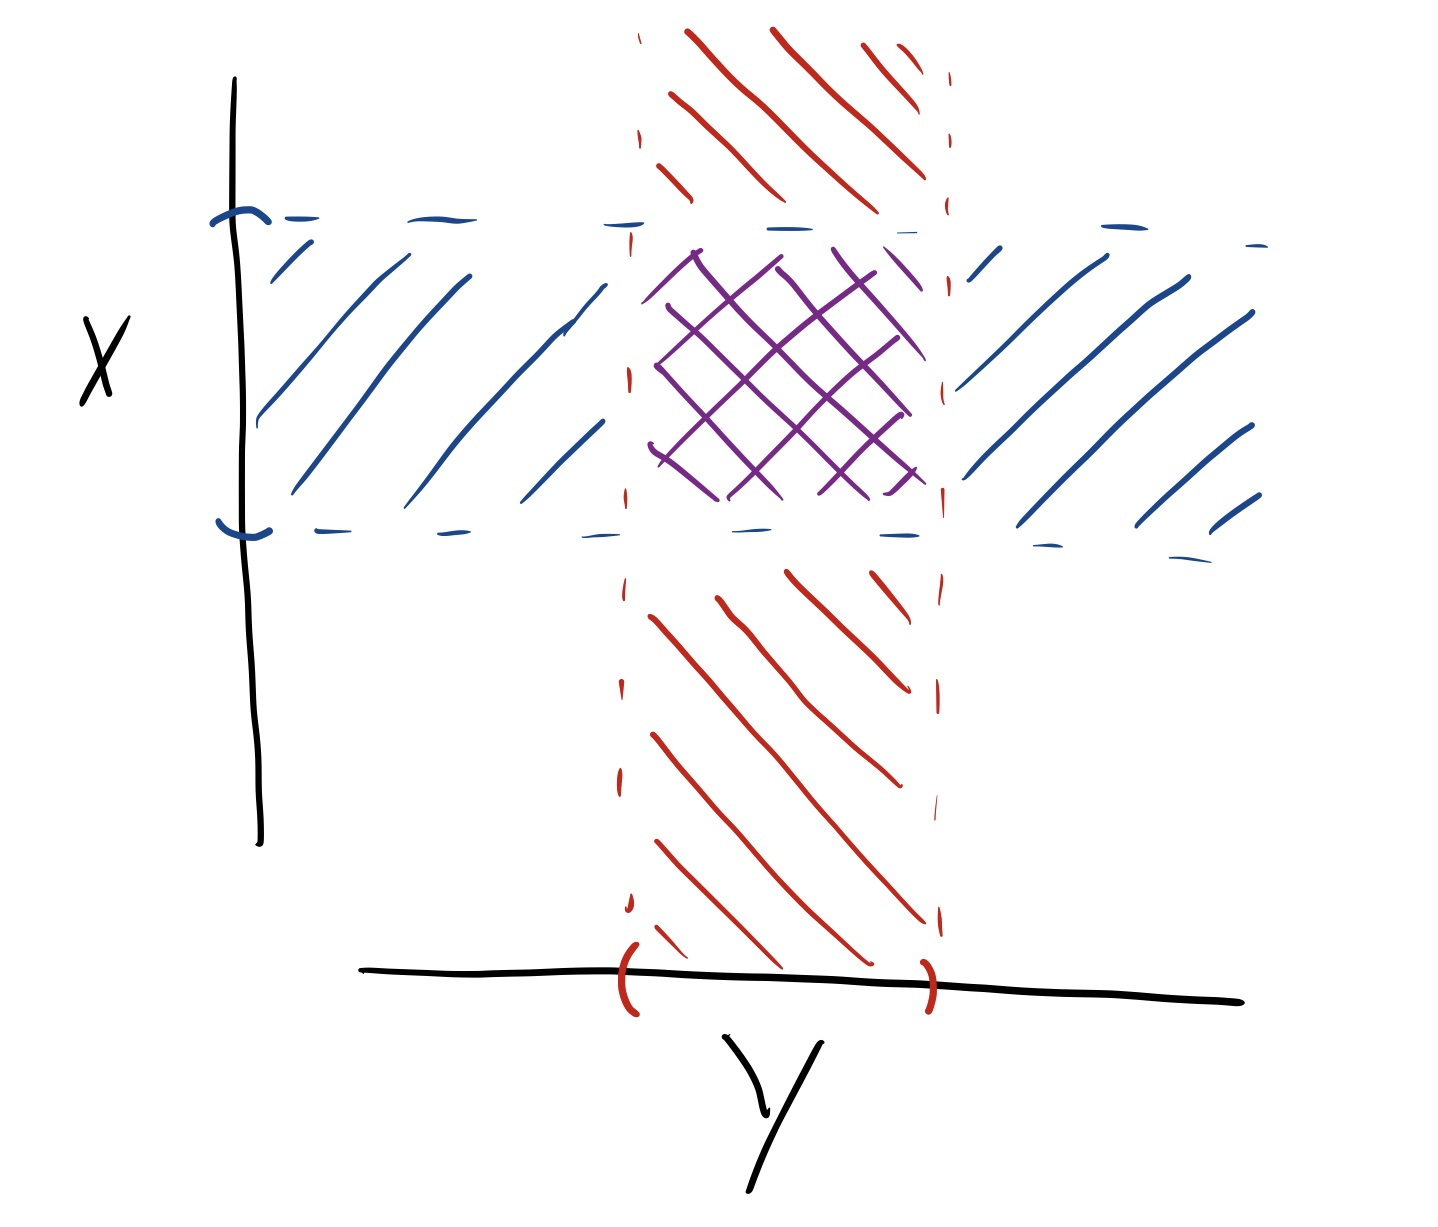
\includegraphics[width=.5\textwidth]{ProductTop}
      \caption{A diagram outlining what our ``Product space'' should look like}
      \label{fig:prodTop}
    \end{figure}
    This is not yet a topology, we still need finite intersections. So, lets add in finite intersections: \(\mathcal{B} = \opn U \times V \stbar U \subseteq X\ \mathrm{open}, V \subseteq Y\ \mathrm{open} \cls\). This in and of itself is still not a topology, but it is a basis.

    \begin{prop}
      Let \(X, Y\) be topological spaces, then the set:
      \begin{align*}
        \mathcal{B} = \opn U \times V \stbar U \subseteq X\ \mathrm{open}, V \subseteq Y\ \mathrm{open} \cls
      \end{align*}
    \end{prop}

    \begin{df}
      The \textbf{product topology on \(X \times Y\)} is the topology generated by the basis \(\mathcal{B}\) above.
    \end{df}

    \begin{exa}
      \(\R^2\) with the usual topology has the product topology from \(\R \times \R\). With the usual topology, we were taking a basis of open balls, but in this construction, we are doing it with open rectangles, which we previously showed was equivalent.
    \end{exa}
\end{document}
%%% Local Variables:
%%% mode: latex
%%% TeX-master: t
%%% End:
